\documentclass{report}

\usepackage{listings, color, graphicx}
\usepackage[spanish]{babel}

\definecolor{dkgreen}{rgb}{0,0.6,0}
\definecolor{gray}{rgb}{0.5,0.5,0.5}
\definecolor{mauve}{rgb}{0.58,0,0.82}

\lstset{
  frame=tb,
  language=java,
  aboveskip=3mm,
  belowskip=3mm,
  showstringspaces=false,
  columns=flexible,
  basicstyle={\small\ttfamily},
  numbers=none,
  numberstyle=\tiny\color{gray},
  keywordstyle=\color{blue},
  commentstyle=\color{dkgreen},
  stringstyle=\color{mauve},
  breaklines=true,
  breakatwhitespace=true,
  tabsize=3
}

\begin{document}
\lstloadlanguages{java,xml}

\begin{titlepage}

	\centering
	
\includegraphics[width=0.5\textwidth]{../images/ciateq.jpg}\par\vspace{1cm}
	\vspace{1cm}
	{\scshape\Large Pr\'{a}ctica de Android\par}
	\vspace{1.5cm}
	{\huge\bfseries Env\'{i}o de par\'{a}metros entre actividades\par}
	\vspace{2cm}
	{\Large\itshape H. Edmundo Ram\'{i}rez\par}
	\vfill
	Profesor\par
	\textsc{Mtro. Jayro Santiago Paz}
	\vfill

% Bottom of the page
	{\large \date sOctubre 2017\par}
\end{titlepage}

\section{Introducci\'{o}n}
Esta pr\'{a}ctica muestra c\'{o}mo pasar parámetros entre actividades (o pantallas) de una aplicaci\'{o}n de Android

\chapter{C\'{o}digos}
\section{MainActivity.java}
\begin{lstlisting}[language=java]
package sim.hecmundo.passing_parameters;

import android.content.Intent;
import android.os.Bundle;
import android.support.v7.app.AppCompatActivity;
import android.view.View;
import android.widget.EditText;

public class MainActivity extends AppCompatActivity {

    @Override
    protected void onCreate(Bundle savedInstanceState) {
        super.onCreate(savedInstanceState);
        setContentView(R.layout.activity_main);
    }

    public void open_act2(View view){
        Intent i= new Intent(this,Main2Activity.class);
        EditText name = (EditText)findViewById(R.id.editText);
        String param = (String) name.getText().toString();
        i.putExtra("name",param);
        startActivity(i);
    }
}
\end{lstlisting}	

Main2Activity.java
\begin{lstlisting}[language=java]
package sim.hecmundo.passing_parameters;

import android.os.Bundle;
import android.support.v7.app.AppCompatActivity;
import android.view.View;
import android.widget.TextView;

public class Main2Activity extends AppCompatActivity {



    @Override
    protected void onCreate(Bundle savedInstanceState) {
        super.onCreate(savedInstanceState);
        setContentView(R.layout.activity_main2);
        TextView nombre = (TextView)findViewById(R.id.textView3);
        String param = getIntent().getStringExtra("name");
        nombre.setText(param);
    }



    public void open_act1(View view) {
        finish();
    }
}
\end{lstlisting}

activity\_main.xml
\begin{lstlisting}[language=xml]
<?xml version="1.0" encoding="utf-8"?>
<android.support.constraint.ConstraintLayout xmlns:android="http://schemas.android.com/apk/res/android"
    xmlns:app="http://schemas.android.com/apk/res-auto"
    xmlns:tools="http://schemas.android.com/tools"
    android:layout_width="match_parent"
    android:layout_height="match_parent"
    tools:context="sim.hecmundo.passing_parameters.MainActivity">

    <EditText
        android:id="@+id/editText"
        android:layout_width="293dp"
        android:layout_height="88dp"
        android:layout_marginBottom="8dp"
        android:layout_marginLeft="8dp"
        android:layout_marginRight="8dp"
        android:layout_marginTop="8dp"
        android:ems="10"
        android:hint="What´s your name?"
        android:inputType="textPersonName"
        android:textAppearance="@android:style/TextAppearance.Holo.Medium"
        android:textSize="30sp"
        app:layout_constraintBottom_toBottomOf="parent"
        app:layout_constraintHorizontal_bias="0.503"
        app:layout_constraintLeft_toLeftOf="parent"
        app:layout_constraintRight_toRightOf="parent"
        app:layout_constraintTop_toTopOf="parent"
        app:layout_constraintVertical_bias="0.276"
        tools:layout_editor_absoluteY="88dp" />

    <Button
        android:id="@+id/button"
        android:layout_width="191dp"
        android:layout_height="135dp"
        android:layout_marginBottom="8dp"
        android:layout_marginLeft="8dp"
        android:layout_marginRight="8dp"
        android:layout_marginTop="61dp"
        android:background="@android:drawable/ic_delete"
        android:onClick="open_act2"
        android:text="Don´t touch"
        android:textAppearance="@android:style/TextAppearance.Holo.Medium"
        android:textSize="24sp"
        android:textStyle="bold"
        app:layout_constraintBottom_toBottomOf="parent"
        app:layout_constraintHorizontal_bias="0.502"
        app:layout_constraintLeft_toLeftOf="parent"
        app:layout_constraintRight_toRightOf="parent"
        app:layout_constraintTop_toBottomOf="@+id/editText"
        app:layout_constraintVertical_bias="0.0" />

</android.support.constraint.ConstraintLayout>

\end{lstlisting}

activity\_main2.xml
\begin{lstlisting}
<?xml version="1.0" encoding="utf-8"?>
<android.support.constraint.ConstraintLayout xmlns:android="http://schemas.android.com/apk/res/android"
    xmlns:app="http://schemas.android.com/apk/res-auto"
    xmlns:tools="http://schemas.android.com/tools"
    android:layout_width="match_parent"
    android:layout_height="match_parent"
    tools:context="sim.hecmundo.passing_parameters.Main2Activity">

    <TextView
        android:id="@+id/textView3"
        android:layout_width="wrap_content"
        android:layout_height="wrap_content"
        android:layout_marginBottom="8dp"
        android:layout_marginLeft="8dp"
        android:layout_marginRight="8dp"
        android:layout_marginTop="8dp"
        android:hint="culpable"
        android:textAppearance="@android:style/TextAppearance.Holo.Large"
        android:textColor="@android:color/holo_orange_dark"
        android:textSize="36sp"
        app:layout_constraintBottom_toBottomOf="parent"
        app:layout_constraintHorizontal_bias="0.513"
        app:layout_constraintLeft_toLeftOf="parent"
        app:layout_constraintRight_toRightOf="parent"
        app:layout_constraintTop_toTopOf="parent" />

    <TextView
        android:id="@+id/textView"
        android:layout_width="wrap_content"
        android:layout_height="wrap_content"
        android:layout_marginBottom="8dp"
        android:layout_marginLeft="8dp"
        android:layout_marginRight="8dp"
        android:layout_marginTop="8dp"
        android:text="Toll you not to touch"
        android:textColor="@android:color/holo_red_dark"
        android:textSize="36sp"
        android:textStyle="bold"
        app:layout_constraintBottom_toBottomOf="parent"
        app:layout_constraintLeft_toLeftOf="parent"
        app:layout_constraintRight_toRightOf="parent"
        app:layout_constraintTop_toTopOf="parent"
        app:layout_constraintVertical_bias="0.294" />

    <Button
        android:id="@+id/button2"
        android:layout_width="wrap_content"
        android:layout_height="wrap_content"
        android:layout_marginBottom="8dp"
        android:layout_marginLeft="8dp"
        android:layout_marginRight="8dp"
        android:layout_marginTop="8dp"
        android:onClick="open_act1"
        android:text="Sorry and Bye"
        android:textColor="@color/colorPrimaryDark"
        android:textSize="14sp"
        android:textStyle="bold"
        app:layout_constraintBottom_toBottomOf="parent"
        app:layout_constraintLeft_toLeftOf="parent"
        app:layout_constraintRight_toRightOf="parent"
        app:layout_constraintTop_toTopOf="parent"
        app:layout_constraintVertical_bias="0.782" />

</android.support.constraint.ConstraintLayout>

\end{lstlisting}

\chapter{Im\'{a}genes}
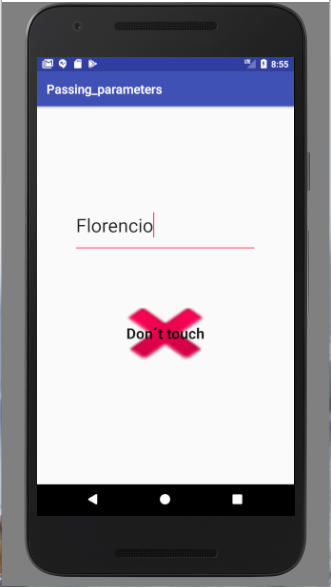
\includegraphics[width=0.5\textwidth]{../images/param_1.PNG}
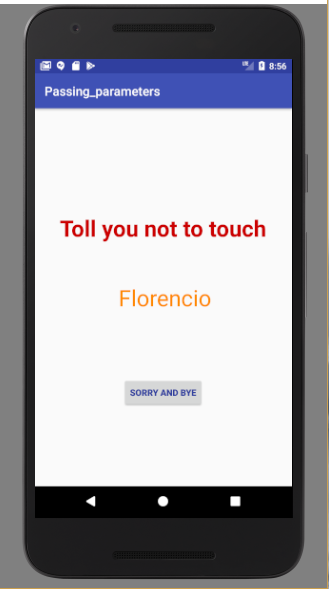
\includegraphics[width=0.5\textwidth]{../images/param_2.PNG}

\end{document}

